\documentclass{report}
% PACKAGES
\usepackage[utf8]{inputenc}
\usepackage{mathtools} % math and figures
\usepackage{float} % make figure appear where we want with [H]
\usepackage{filecontents}
\usepackage[numbered,framed]{matlab-prettifier}
% these packages include more math symbols you might use
\usepackage{amsmath,amsfonts,amsthm,amssymb}


% PROJECT Specific Information to Fill Out
\newcommand{\LectureDate}{\today}
\newcommand{\LectureClassName}{Problem Set 3}
\newcommand{\LatexerName}{SeungWha Lee, Xinyuan Meng, Boyang Pan}
\author{\LatexerName}


% CONFIGURATIONS to make the report look better
\usepackage{setspace}
\usepackage{Tabbing}
\usepackage{fancyhdr}
\usepackage{lastpage}
\usepackage{extramarks}
\usepackage{afterpage}
\usepackage{abstract}

% In case you need to adjust margins:
\topmargin=-0.45in
\evensidemargin=0in
\oddsidemargin=0in
\textwidth=6.5in
\textheight=9.0in
\headsep=0.25in

% Setup the header and footer
\pagestyle{fancy}
\lhead{\LatexerName}
\rhead{\LectureDate}
\lfoot{\lastxmark}
\cfoot{}
\rfoot{Page\ \thepage\ of\ \pageref{LastPage}}
\renewcommand\headrulewidth{0.4pt}
\renewcommand\footrulewidth{0.4pt}
\renewcommand\thesection{\arabic{section}}
\renewcommand{\thesubsection}{\thesection.\Alph{subsection}}
\usepackage{color}

\title{\LectureTitle: Assignment 2}

\begin{document}
\maketitle
\newpage

\section{Exercise 1}
In this Exercise,  $R$ is the mean of returns on 10 industries ($N\times1$ matrix), $\sigma$ is the standard deviation of returns on 10 industries ($N\times1$ matrix), $V$ is the covariance matrix ($N\times N$ matrix) and $\mathbf{1}$ is (1 1 ... 1)$'$ ($N\times1$ matrix).
\subsection{Part A}
The plot that contains the efficient frontier, the tangency portfolio, the MVP portfolio and the 10 industries are given below. The efficient frontier is parabola, and both the MVP and the Tangency portfolio land on the efficient frontier, but the 10 industries are on the right side of the efficient frontier.

\begin{itemize}
\item For MVP, the weights for individual assets are $W_{MVP} = \frac{V^{-1}\mathbf{1}}{\mathbf{1}'V^{-1}\mathbf{1}}$.
\subitem - Based on the given dataset, $W_{MVP}$ = 
\[
\begin{bmatrix}
    76.88\% & -5.73\% & -13.72\% & 21.83\% & -10.56\% & 54.94\% & -5.58\% & 7.13\% & 7.32\% & -32.52\%
\end{bmatrix}
\]
\subitem  - $r_{MVP} = RW_{MVP}= 0.9204\%$,  $\sigma_{MVP} = W_{MVP}'VW_{MVP}= 3.7286\%$.
\item For TP, the weights for individual assets are $W_{TP} = \frac{V^{-1}(R-r_f\mathbf{1})}{\mathbf{1}'V^{-1}(R-r_f\mathbf{1})}$ given $V$ is the covariance matrix and $\mathbf{1}$ is (1 1 ... 1)$'$ ($N\times1$ matrix).\textcolor{red}{diff from BW's formula}
\subitem - Based on the given dataset, $W_{TP}$ = 
\[
\begin{bmatrix}
    83.77\% & 7.99\% & -17.61\% & 32.05\% & 3.19\% & 33.32\% & -4.70\% & 28.18\% & -3.43\% & -62.76\%
\end{bmatrix}
\]
\subitem - $r_{TP} = RW_{TP}= 1.0320\%$,  $\sigma_{TP} = W_{TP}'VW_{TP}= 4.0395\%$.
\item The relationship between standard deviations and expected returns on the portfolios on the efficient frontier is $\sigma^2 = (r_p \,\,\, \mathbf{1}) A^{-1} (r_p \,\,\, \mathbf{1})'$ where $A = (R \,\,\, \mathbf{1})' V^{-1} (R \,\,\, \mathbf{1})$($2\times 2$ matrix). Suppose 
\end{itemize}

\begin{figure}[H]
	\centering
	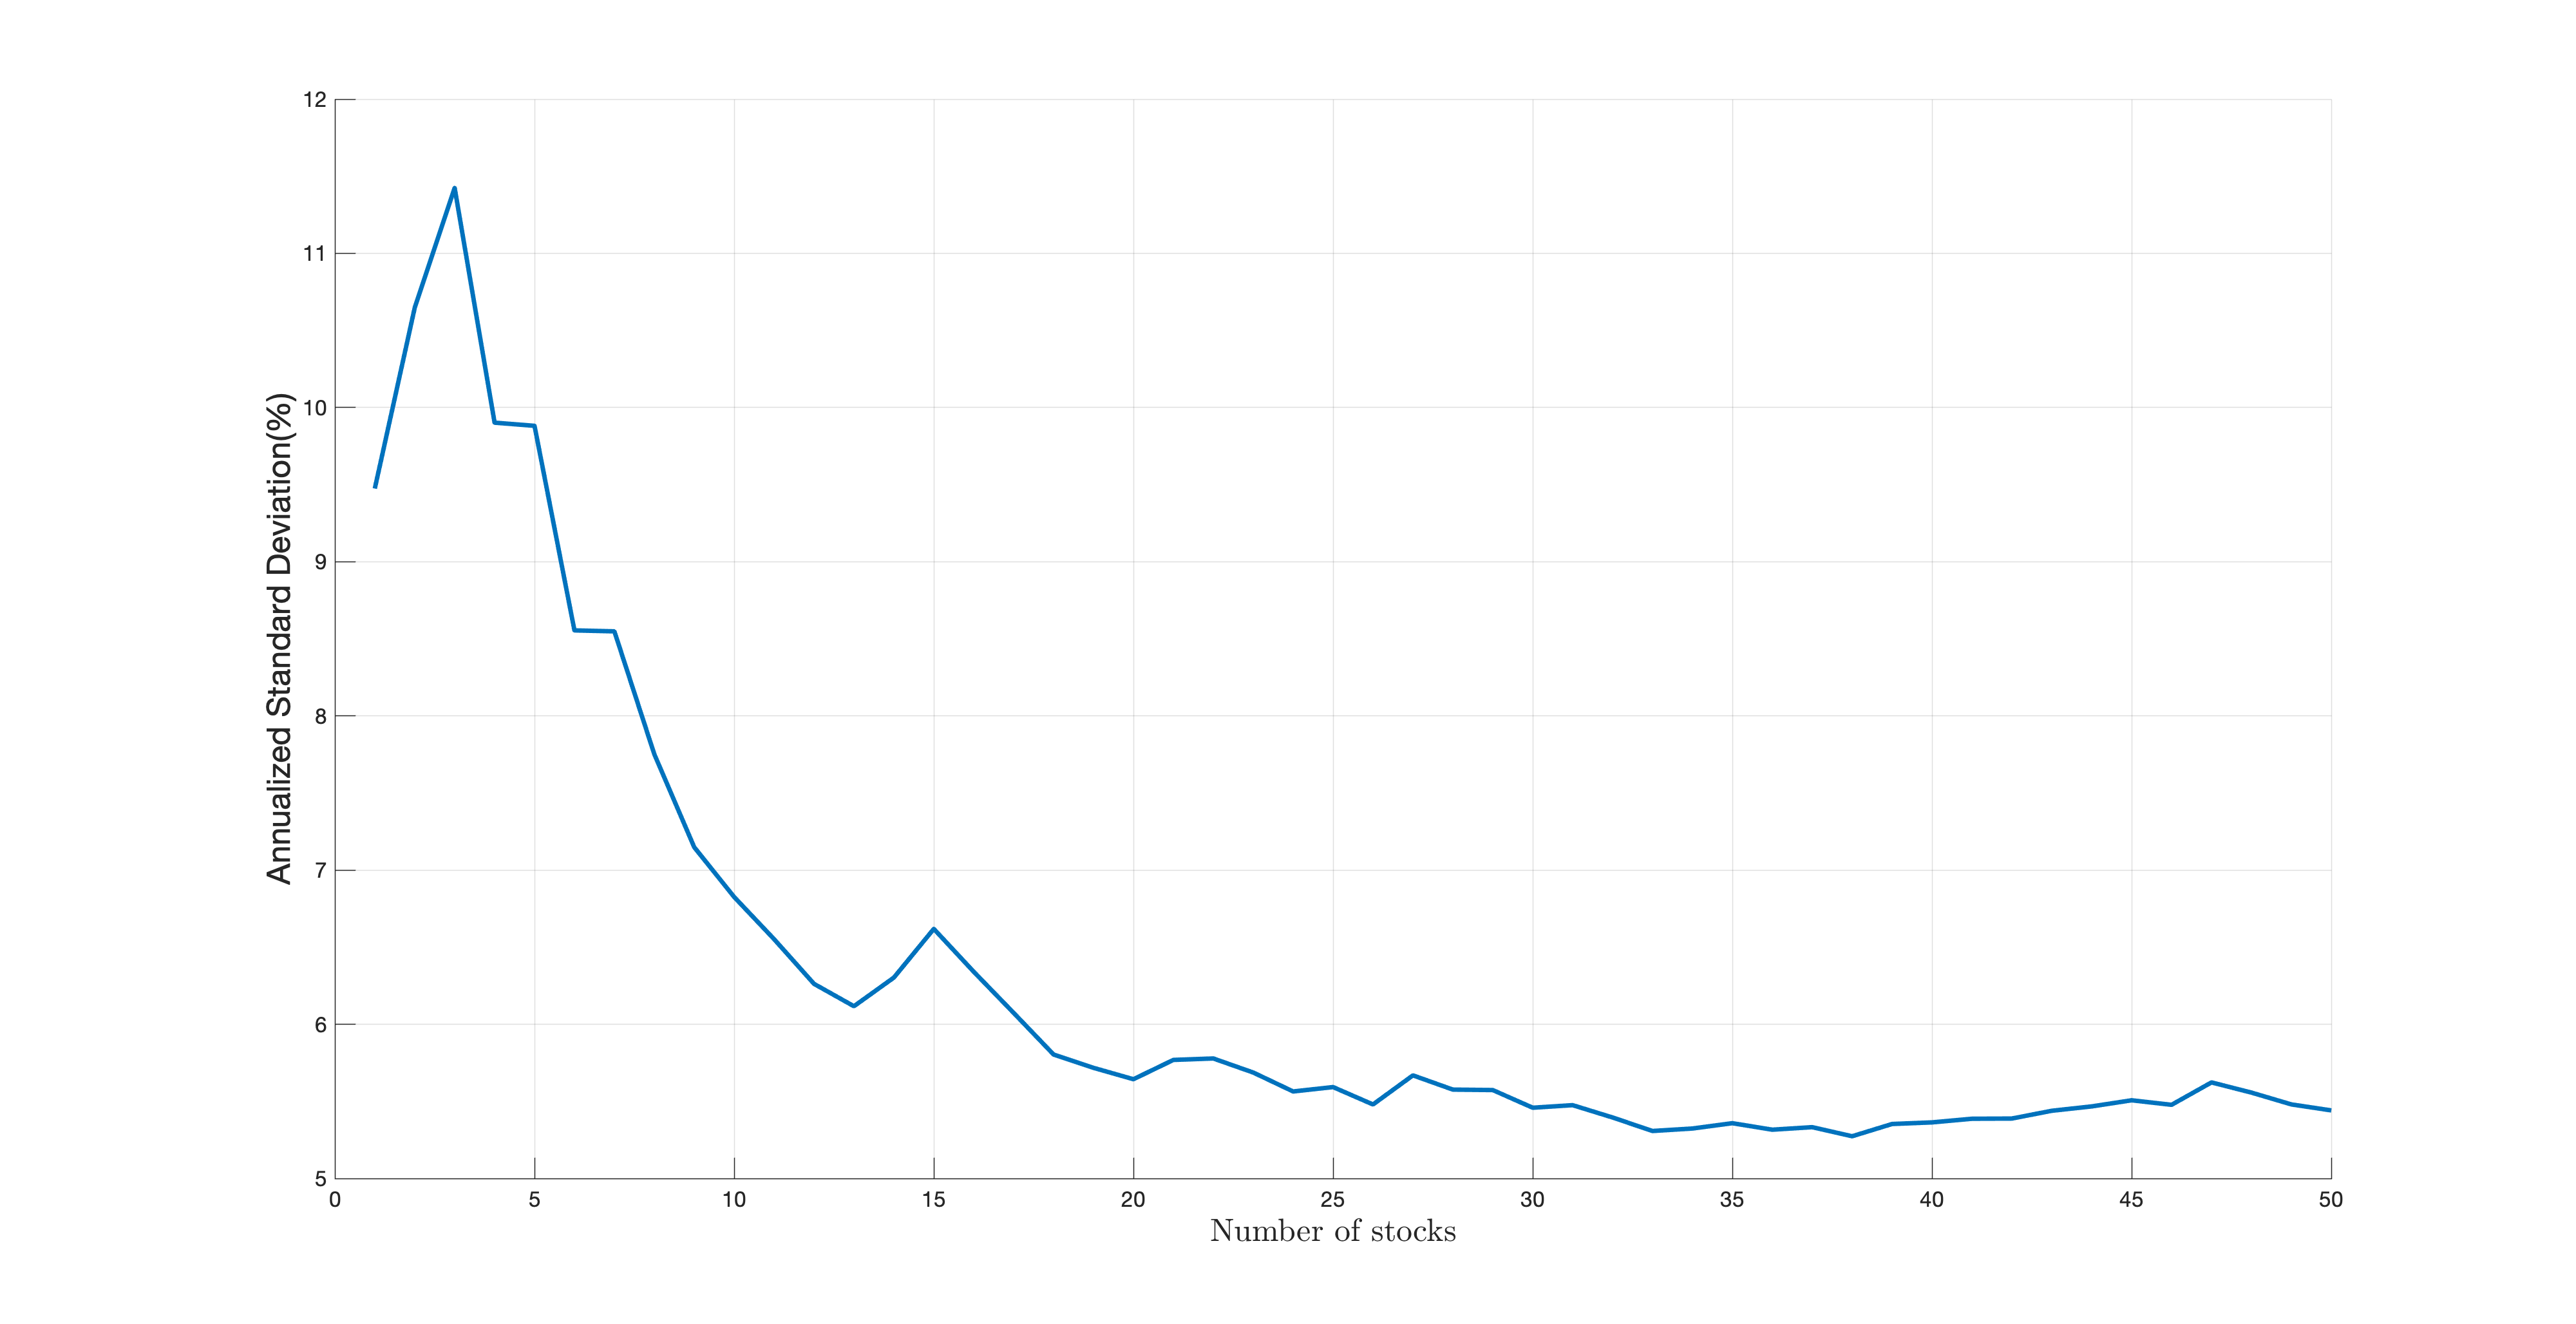
\includegraphics[width=1.0\textwidth]{figures/1A}
	\caption{Efficient Frontier of the 10-industry portfolios}
\end{figure}



\begin{table}[H]
	\centering
	\caption{The means and standard deviations of 4 equal-weight portfolios}
	\begin{tabular}{ccccc}\hline\hline
	Number of Stocks & 5 & 10 & 25 & 50 \\\hline
	Mean & 1.5164 & 1.2326 & 1.2119 & 1.2107 \\
	Standard Deviation & 9.8671 & 6.8118 & 5.5771 & 5.4281 \\ \hline
	\end{tabular}
\end{table}

\end{document}